% Packages
\documentclass[12pt]{article}
\usepackage[margin=2.5cm]{geometry}
\usepackage{lipsum}
\usepackage{titlesec, titletoc}
\usepackage[svgnames, table]{xcolor}
\usepackage{algorithm}
\usepackage{algpseudocode}
\usepackage{mdframed}
\usepackage[T1]{fontenc}
\usepackage{amsmath,amsthm,amsfonts,amssymb,mathtools}
\usepackage[osf]{mathpazo}
\usepackage{enumitem}

% Formating setup
\footskip = 1 cm
\setlength{\parindent}{0pt}
\pdfpxdimen=1in
\parindent = 0pt
\definecolor{myBlue}{RGB}{0, 81, 255}
\titleformat{\section}[block]{\sffamily\large\bfseries}{\thesection}{.5em}{\textcolor{myBlue}
{\titlerule[1.5pt]}\\\sffamily}[\vspace*{-3mm}\textcolor{myBlue}{\titlerule[1.5pt]}]
\titleformat{\subsection}{\large\sffamily\bfseries}{\thesubsection}{0.5em}{\textcolor{Black}}
\newcounter{boxedlistcounter}
\newenvironment{pseudo}{%
  \setcounter{boxedlistcounter}{0}% <-- Add this line to reset the counter
  \mdframed[
    linecolor=black, % color of the border
    linewidth=1.5pt, % thickness of the border
    roundcorner=10pt, % radius of the corners
    innertopmargin=0.6\baselineskip, % space at the top of the box
    innerbottommargin=0.6\baselineskip, % space at the bottom of the box
  ]
  \fontsize{12pt}{14pt}\selectfont % add font size command here
  \mdseries % add font series command here
}{%
  \endmdframed%
}
\newcommand{\I}{\par\stepcounter{boxedlistcounter}\arabic{boxedlistcounter}.\hspace{5pt}}
\newcounter{boxedlistcounter2}
\newenvironment{Proof}{%
  \refstepcounter{boxedlistcounter2}%
  \mdframed[
    linecolor=black, % color of the border
    linewidth=1.5pt, % thickness of the border
    roundcorner=10pt, % radius of the corners
    innertopmargin=\baselineskip, % space at the top of the box
    innerbottommargin=\baselineskip, % space at the bottom of the box
  ]
  \fontsize{12pt}{14pt}\selectfont % add font size command here
  \mdseries % add font series command here
}{%
  \endmdframed%
}
\newcommand{\PI}{\par\textbullet\hspace{5pt}}
\setlist[itemize]{itemsep=1pt}
\newcommand{\NL}{\par\hspace{12.5pt}}
\setlist[itemize]{itemsep=1pt}

% Custom commands
\newcommand{\for}[1]{\textbf{for} #1 \textbf{do}}
\newcommand{\IF}[1]{\textbf{if} #1 \textbf{then}}
\newcommand{\ELIF}[1]{\textbf{else if} #1 \textbf{then}}
\newcommand{\ELSE}{\textbf{else}}
\newcommand{\return}[1]{\textbf{return} #1}
\newcommand{\assign}{ $\leftarrow$ }
\newcommand{\DEF}[2]{\textbf{def} #1(#2):}
\newcommand{\1}{\space \quad}
\newcommand{\2}{\quad \quad \quad}
\newcommand{\3}{\quad \quad \quad \quad \space}
\newcommand{\4}{\quad \quad \quad \quad \quad \quad}
\newcommand{\5}{\quad \quad \quad \quad \quad \quad \quad \space}
\newcommand{\comment}[1]{\hfill \textit{\# #1}}
\newcommand{\while}[1]{\textbf{while} #1 \textbf{do}}

% Document start ------------------------------------------------------------------------------------
\begin{document}

% Section 1  ----------------------------------------------------------------------------------------
\section{Introduction to Greedy Algorithms}
Greedy alogirthms are a class of algorithms where we build a solution one step at a time
making locally optimal choices at each stage in the hope of finding a global optimum solution.
So no back tracking is done.
\begin{pseudo}
  \I \DEF{GreedyAlgorithm}{input}
  \I \1 initalise result \comment{initalisation}
  \I \1 determine order in which to consider input
  \I \1 \for{each element i of the input (in abover order)} \comment{make greedy choices}
  \I \2 \1 \IF{element i improves result}
  \I \3 update result with element i
  \I \1 \return{result}
\end{pseudo}

\subsection{The Fractional Knapsack Problem}
Given a set S of n items, with each item i having $b_i$ (a positive benefit) and $w_i$ (a positive weight),
and a knapsack of capacity W, find a subset of S that maximises the total benefit of the items in the subset.
Let $x_i$ denote the amount we take of item i.

\vspace{10pt}
\textbf{Required to maximise:} $\sum_{i \in S} b_i(x_i/w_i)$
\begin{pseudo}
  \I \DEF{FractionalKnapsack}{b, w, W}
  \I \1 x \assign array of size |b| of zeros \comment{initalisation}
  \I \1 current \assign $0$
  \I \1 \for{i in descending b[i]/w[i] order} \comment{make greedy choices}
  \I \2 x[i] \assign min(w[i], W - current) \comment{Don't take more than we can}
  \I \2 current \assign current + x[i]
  \I \1 \return{x}
\end{pseudo}
Require O(n log n) time to sort the items and then O(n) time to process them in the for-loop.

\subsection{Task scheduling}
Given a set of n lectures, each with a start time $s_i$ and finish time $f_i$, find the minimum number
of classrooms required to schedule all lectures so that no two occur at the same time in the same room.

\vspace{10pt}
The depth of a set of open intervals is the maximum number that contain any given time. Therefore, the number
of classrooms needed $\geq$ depth of the set of intervals.
\begin{pseudo}
  \I \DEF{TaskScheduling}{S} \comment{O(n log n)}
  \I \1 sort S by increasing startng time order \comment{initalisation}
  \I \1 rooms \assign 0
  \I \1 \for{each lecture i in S} \comment{make greedy choices}
  \I \2 \IF{lecture i is compatible with some classroom k}
  \I \3 schedule lecture i in classroom i $\leq$ k $\leq$ d
  \I \2 \ELSE
  \I \3 allocate a new classroom rooms + 1
  \I \3 schedule lecture i in classroom rooms + 1
  \I \3 rooms \assign rooms + 1
  \I \1 \return{rooms}
\end{pseudo}

\vspace{10pt}
\textbf{RTP:} Greedy algorithm is optimal
\begin{Proof}
  \PI rooms = number of classrooms that the greedy algorithm allocates.
  \PI Classroom rooms is opened because we needed to schedule a job, say i, that is 
  \NL incompatible with all rooms-1 other classrooms.
  \PI Since we sorted by start time, all these incompatibilities are caused by lectures that 
  \NL start no later than $s_i$. 
  \PI Thus, we have rooms lectures overlapping at time $s_i$.
  \PI All schedules use $\geq$ rooms classrooms. 
\end{Proof}

% Section 2  ----------------------------------------------------------------------------------------
\section{Text Compression}
Given a string X, efficiently encode X into a smaller string Y that saves memory and/or bandwith.

\subsection{Encoding Trees}
A binary code is a mapping of each character of an alphabet to a binary code-word. A prefix code is a code 
such that no code-word is the prefix of another code-word. An encoding tree represents a prefix code, whereby
each external node stores a character and the code word of a character is the path from the root to the external
node.
\begin{center}
  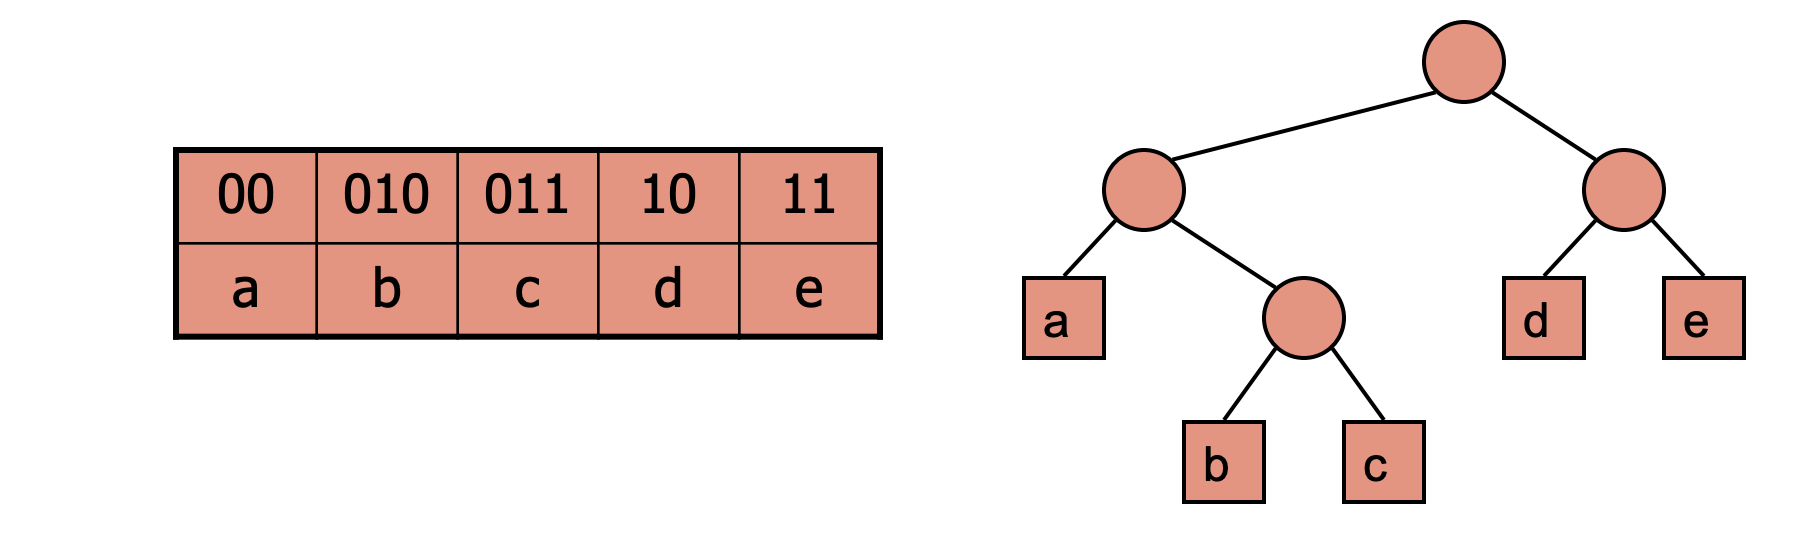
\includegraphics[width=0.8\textwidth]{image26.png}
\end{center}

\subsection{Huffman encoding - Encoding Tree Optimization}
\begin{itemize}
  \item Let C be the set of characters in X.
  \item Compute frequency f(c) for each character c in C.
  \item Encode high-frequency characters with short codes and low-frequency characters with long codes.
  \item No code word is a prefix of another code word.
  \item Use an optimal encoding tree to determine the code words.
\end{itemize}

Given a string X, Huffman’s algorithm constructs a prefix code that minimizes the size of the encoding of X.
It runs in time O(n + d log d), where n is the size of X and d is the number of distinct characters of X.
The algorithm builds the encoding tree from the bottom up, merging trees as it goes along, using a priority 
queue to guide the process.

\vspace{10pt}
$$\text{\textbf{Minimises: }} \sum_{c \in C} f(c) \times \text{depth of c in tree}$$

\begin{pseudo}
  \I \DEF{Huffman}{C, f} \comment{O(|C|log|C|)}
  \I \1 Q \assign priority queue of C \comment{initalisation}
  \I \1 \for{c in C}
  \I \2 T \assign single-node binary tree storing c
  \I \2 insert T into Q with key f(c)
  \I \1 \while{Q.size() > 1} \comment{make greedy choices}
  \I \2 $f_1$, $T_1$ \assign Q.removeMin()
  \I \2 $f_2$, $T_2$ \assign Q.removeMin()
  \I \2 $T$ \assign new binary tree with $T_1$ and $T_2$ as left and right subtrees.
  \I \2 f \assign $f_1$ + $f_2$
  \I \2 insert T into Q with key f
  \I \1 \return{Q.removeMin()} \comment{returns encoding tree}
\end{pseudo}
\begin{center}
  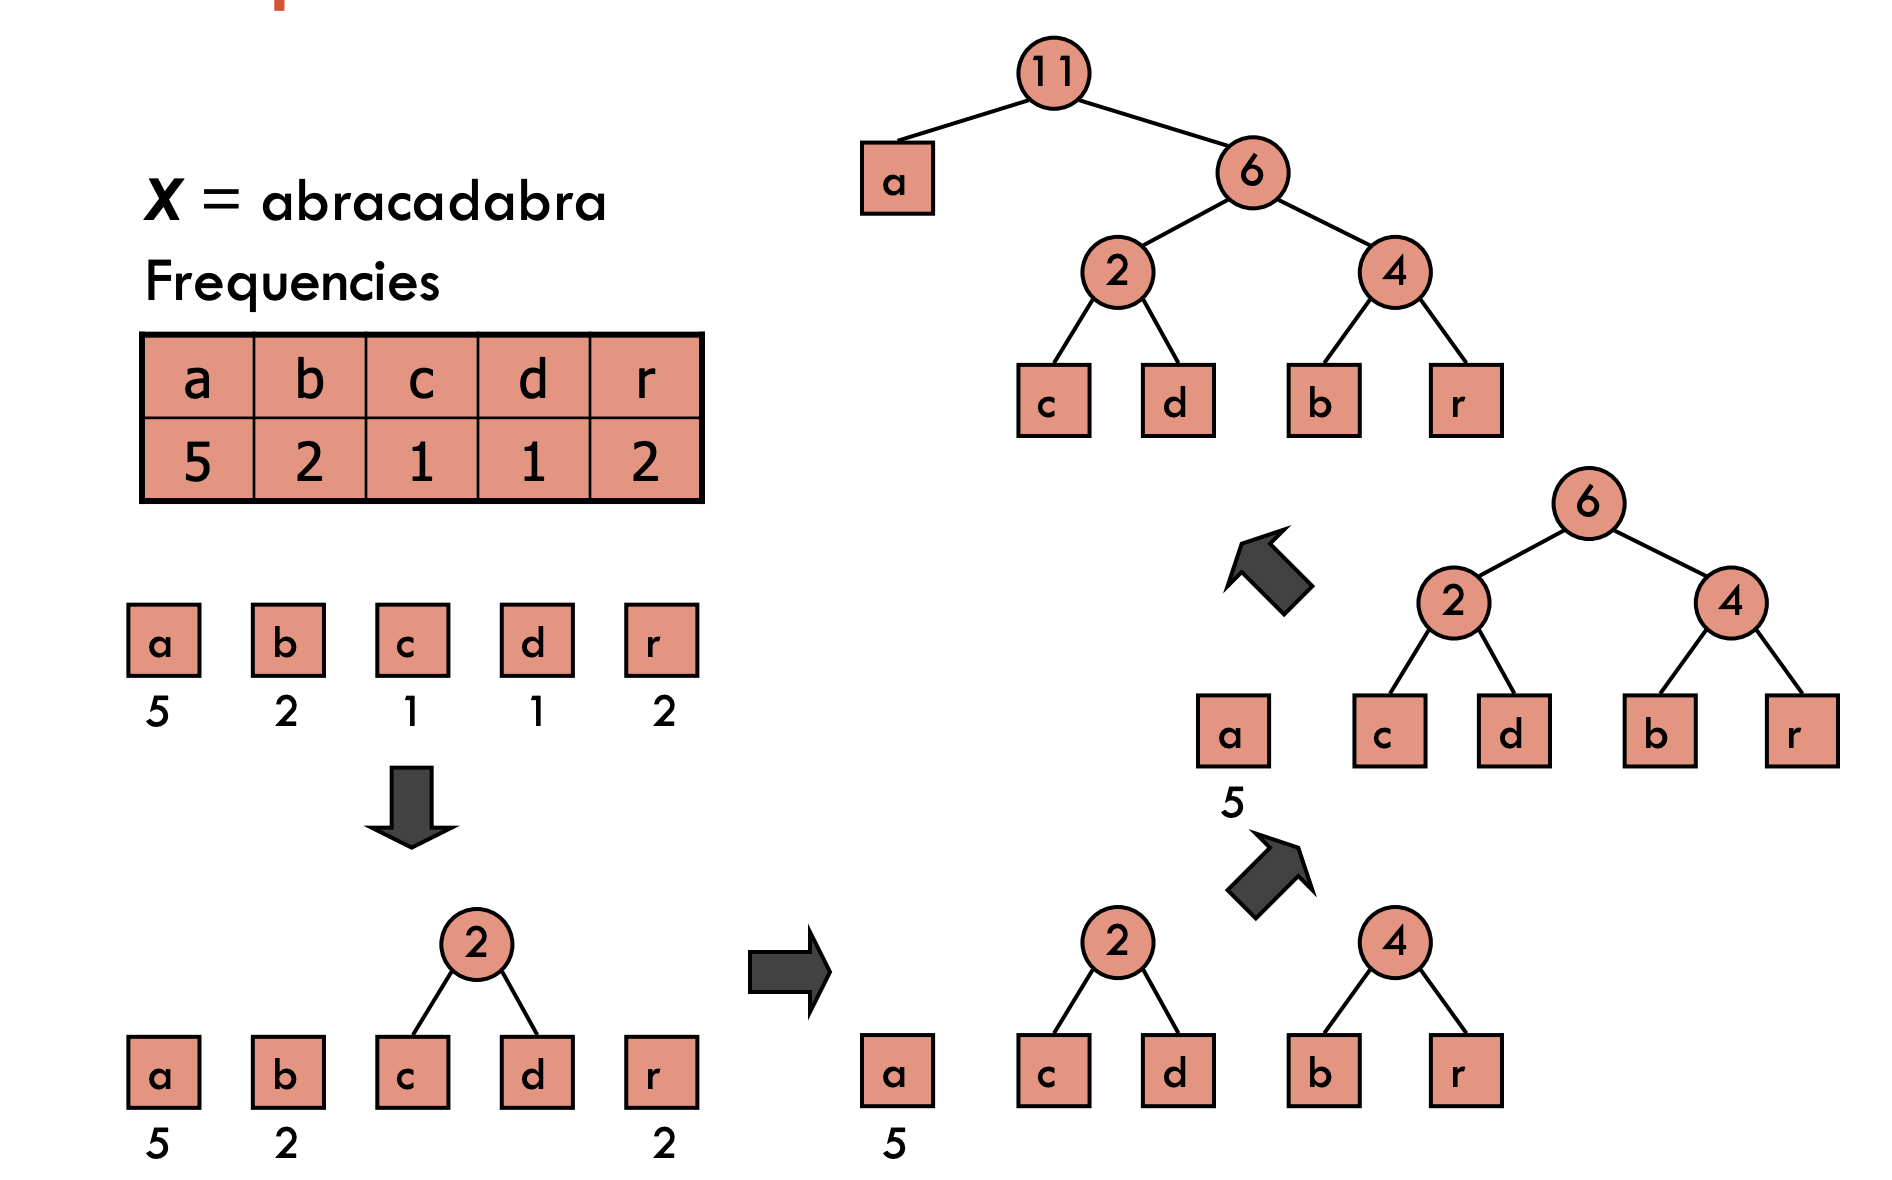
\includegraphics[width=0.7\textwidth]{image27.png}
\end{center}
\end{document}